%% IEEE Double-Column Style
%% Cattle Pinkeye (Infectious Bovine Keratoconjunctivitis) Detection
%% via a Two-Stage Deep Learning Pipeline

\documentclass[10pt,journal,compsoc]{IEEEtran}

\usepackage[T1]{fontenc}
\usepackage[utf8]{inputenc}
\usepackage{amsmath,amssymb}
\usepackage{graphicx}
\usepackage{booktabs}
\usepackage{multirow}
\usepackage{array}
\usepackage{xcolor}
\usepackage{hyperref}
\usepackage{float}
\usepackage{cite}
\usepackage{url}
\usepackage{tikz}
\usetikzlibrary{arrows.meta, positioning, shapes.geometric}

\hypersetup{
  colorlinks=true,
  linkcolor=blue,
  citecolor=blue,
  urlcolor=blue
}

\newcolumntype{C}[1]{>{\centering\arraybackslash}m{#1}}

\begin{document}

\title{A Two-Stage Deep Learning Pipeline for Automated Detection of
Infectious Bovine Keratoconjunctivitis in Cattle}

\author{%
  \IEEEauthorblockN{Iman Khazrak}\\
  \IEEEauthorblockA{Department of Computer Science\\
    University Name\\
    Email: \texttt{imankhazrak@university.edu}}
}

\maketitle

\begin{abstract}
Infectious bovine keratoconjunctivitis (IBK), commonly known as pinkeye,
is a highly contagious ocular disease in cattle that causes significant
welfare and economic losses. Early automated detection from farm images
can enable timely veterinary intervention. We present a two-stage deep
learning pipeline: \emph{Stage~1} localises the eye region using a
YOLOv8 detector, and \emph{Stage~2} classifies the cropped eye as
healthy or diseased using four architectures---ResNet18,
EfficientNet-B0, a baseline CNN+Transformer hybrid, and an enhanced
CNN+Transformer variant with a class token and deeper head.
Evaluated on 394 labelled eye crops (309 healthy, 85 pinkeye) under
stratified 5-fold cross-validation, the Strong CNN+Transformer achieves
the highest mean accuracy (95.94\,\%) and the highest mean F1-score on
the minority pinkeye class (90.51\,\%); ResNet18 attains the highest
mean ROC-AUC (98.67\,\%) among the four models in the primary benchmark.
Augmentation ablations show architecture-dependent gains and trade-offs.
These results support eye-localised classification as a feasible screen
for this imbalanced, fine-grained imaging setting.
\end{abstract}

\begin{IEEEkeywords}
Pinkeye detection, YOLOv8, CNN+Transformer, class imbalance,
data augmentation, cattle health monitoring, transfer learning.
\end{IEEEkeywords}

\section{Methodology}
\label{sec:methodology}

\subsection{Overview of the Pipeline}
\label{subsec:overview}

The proposed system is a two-stage cascaded pipeline, illustrated in
Fig.~\ref{fig:pipeline}. In the first stage a YOLOv8-based object
detector localises the eye region in each cattle head image. The
detected bounding box is padded and cropped, producing a standardised
eye-region image that forms the input to Stage~2. In the second stage,
four deep classification models are trained and evaluated on the cropped
eye images to discriminate between healthy eyes and eyes affected by IBK.

\begin{figure}[t]
  \centering
  \resizebox{0.92\linewidth}{!}{%
  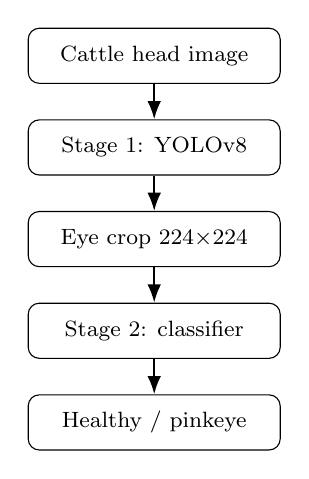
\begin{tikzpicture}[
      font=\footnotesize,
      node distance=4.5mm,
      >=Latex,
      box/.style={
        rectangle,
        draw,
        rounded corners,
        align=center,
        minimum width=3.2cm,
        minimum height=7mm,
        inner sep=3pt
      }
    ]
    \node[box] (img) {Cattle head image};
    \node[box, below=of img] (det) {Stage 1: YOLOv8};
    \node[box, below=of det] (crop) {Eye crop $224{\times}224$};
    \node[box, below=of crop] (cls) {Stage 2: classifier};
    \node[box, below=of cls] (out) {Healthy / pinkeye};
    \draw[->, thick] (img) -- (det);
    \draw[->, thick] (det) -- (crop);
    \draw[->, thick] (crop) -- (cls);
    \draw[->, thick] (cls) -- (out);
  \end{tikzpicture}%
  }
  \caption{High-level two-stage pipeline: localise the eye, then classify
    disease from the cropped region.}
  \label{fig:pipeline}
\end{figure}

\subsection{Dataset}
\label{subsec:dataset}

\subsubsection{Eye Detection Dataset (Stage~1)}
The YOLOv8 detector was trained on 117 cattle head images sourced from
the Roboflow Eye Detection dataset (v3) \cite{roboflow_eye}. Each image
carries a single bounding-box annotation for the \texttt{eye} class in
YOLO normalised format. All 117 annotation files were validated (pairing,
coordinate ranges, class ID${}=0$) prior to training. The dataset was
split deterministically with seed 42 into training (80\,\%, 93 images),
validation (10\,\%, 11 images), and test (10\,\%, 13 images), using the
same stratification rule as in the logged detector training run.

\subsubsection{Classification Dataset (Stage~2)}
The classification pool comprised 408 cattle head images with folder
labels (healthy / pinkeye). After YOLO inference and cropping at
confidence 0.25, 394 images yielded usable eye crops; 14 images had no
passing detection and were set aside for manual review
\cite{advisor_summary}. The Stage~2 dataset therefore contains 309 healthy
and 85 pinkeye crops (78.4\,\% / 21.6\,\%). Images are resized to
$224 \times 224$ for classification.

\subsection{Stage~1: Eye Localisation with YOLOv8}
\label{subsec:stage1}

\subsubsection{Annotation Validation}
The Roboflow export was checked with a validation script (format,
bounds, class ID). All 117 labels passed.

\subsubsection{Detector Training}
A YOLOv8n model pretrained on MS-COCO was fine-tuned on the 93-image
training split using the Ultralytics YOLOv8 API \cite{ultralytics2023yolov8}.
Hyperparameters match the logged training run in the project detector
report (Table~\ref{tab:yolo_config}).

\begin{table}[h]
  \caption{YOLOv8n Training Hyperparameters (Stage~1)}
  \label{tab:yolo_config}
  \centering
  \begin{tabular}{ll}
    \toprule
    \textbf{Parameter} & \textbf{Value} \\
    \midrule
    Base model        & YOLOv8n (pretrained, MS-COCO) \\
    Epochs            & 100 \\
    Image size        & $640 \times 640$ \\
    Batch size        & 16 \\
    Optimizer         & AdamW (framework default LR schedule) \\
    Training images   & 93 \\
    Validation images & 11 \\
    Test images       & 13 \\
    Random seed       & 42 \\
    \bottomrule
  \end{tabular}
\end{table}

\subsubsection{Eye Cropping}
The best detector checkpoint was applied to all 408 classification images
with confidence threshold 0.25 and symmetric padding 10\,\% around each
box (clamped to image bounds), matching the detector inference settings
above (confidence 0.25, 10\,\% symmetric padding).
Figure~\ref{fig:yolo_stage1_example} shows a representative head image
from validation-style inference: the fine-tuned detector places a box on
the eye with a class score, and the crop after padding is the
resolution-matched input to Stage~2.

\begin{figure}[t]
  \centering
  \begin{minipage}[b]{0.48\linewidth}
    \centering
    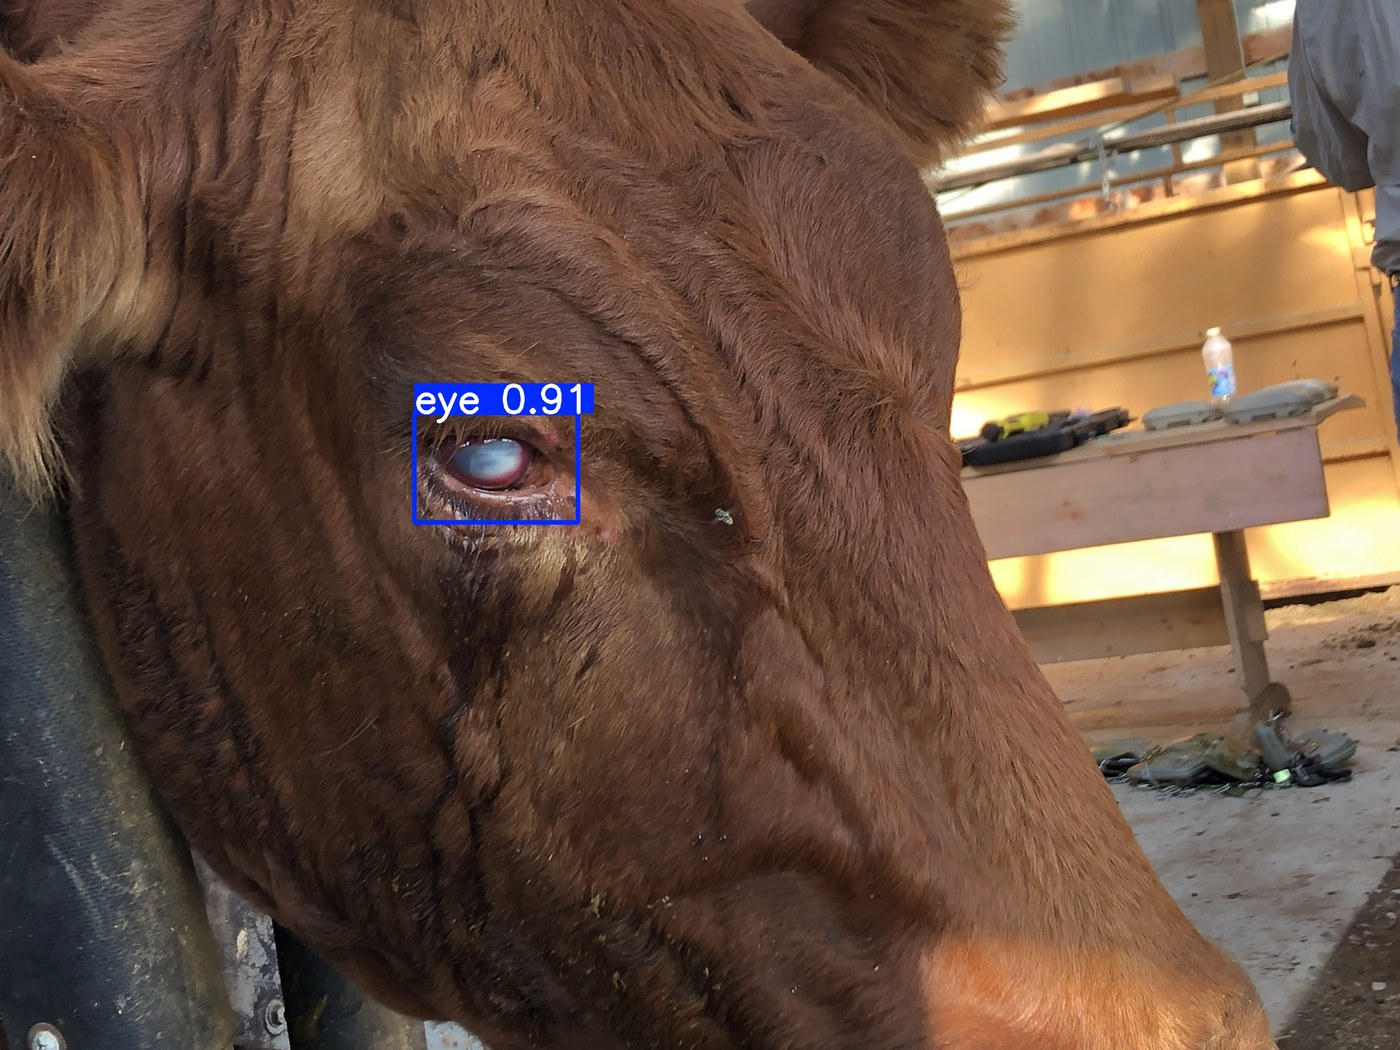
\includegraphics[width=\linewidth]{figures/yolo_eye_detection.jpg}\\[3pt]
    \footnotesize (a) Detection (bounding box and score)
  \end{minipage}
  \hfill
  \begin{minipage}[b]{0.48\linewidth}
    \centering
    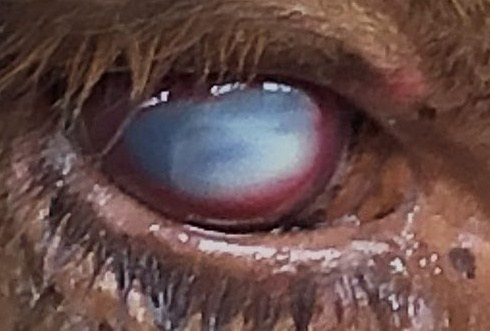
\includegraphics[width=\linewidth]{figures/yolo_eye_crop.jpg}\\[3pt]
    \footnotesize (b) Eye crop fed to classification
  \end{minipage}
  \caption{Qualitative example of Stage~1 localisation after fine-tuning:
    (a)~predicted eye region on a cattle head image; (b)~cropped eye with
    padding, resized to $224\times 224$ before Stage~2.}
  \label{fig:yolo_stage1_example}
\end{figure}

\subsection{Stage~2: Classification Models}
\label{subsec:stage2}

\subsubsection{ResNet18 Baseline}
ResNet18~\cite{he2016resnet} with ImageNet-1k weights was adapted by
replacing the final fully connected layer with a $512 \rightarrow 2$
head and fine-tuning the full network.

\subsubsection{EfficientNet-B0 Baseline}
EfficientNet-B0~\cite{tan2019efficientnet} with ImageNet-1k weights was
adapted with a $1280 \rightarrow 2$ classifier head and end-to-end
fine-tuning.

\subsubsection{Baseline CNN+Transformer Hybrid}
The baseline hybrid feeds final-stage CNN feature maps through a
$1 \times 1$ projection, flattens spatial locations into tokens, applies
a Transformer encoder, mean-pools tokens, and classifies with a linear
head in our implementation.

\subsubsection{Strong CNN+Transformer}
\label{subsubsec:strong}
The Strong variant uses an EfficientNet-B0 backbone (features-only),
$1 \times 1$ projection with BatchNorm and GELU, patch tokens with a
learnable CLS token and learnable positional embeddings, a pre-norm
Transformer encoder ($L{=}3$, $h{=}4$, $d{=}256$), and an MLP classification
head on the CLS output \cite{rw2019timm}. Hyperparameters are summarised
in Table~\ref{tab:strong_config}.

\begin{table}[h]
  \caption{Strong CNN+Transformer Architectural Hyperparameters}
  \label{tab:strong_config}
  \centering
  \begin{tabular}{ll}
    \toprule
    \textbf{Parameter}        & \textbf{Value} \\
    \midrule
    CNN backbone              & EfficientNet-B0 (pretrained) \\
    Embedding dimension $d$   & 256 \\
    Transformer heads $h$     & 4 \\
    Transformer layers $L$    & 3 \\
    MLP ratio                 & 4.0 \\
    Dropout                   & 0.1 \\
    Attention dropout         & 0.1 \\
    Token norm                & Pre-LayerNorm \\
    Activation                & GELU \\
    \bottomrule
  \end{tabular}
\end{table}

\subsection{Training Protocol}
\label{subsec:training}

\subsubsection{Stratified 5-Fold Cross-Validation}
With 394 crops, we used stratified 5-fold cross-validation (seed 42),
preserving the healthy/pink-eye ratio in each fold. Each fold uses four
parts for training and one for validation; metrics are summarised as
mean $\pm$ standard deviation across folds.

\subsubsection{Loss Function and Class Imbalance}
Training used weighted cross-entropy with class weights
$w_c = N / (K n_c)$ over the \emph{training-fold} sample counts (inverse
frequency within each fold). This upweights
the minority pinkeye class relative to healthy samples.

\subsubsection{Optimiser and Early Stopping}
Optimisation used AdamW \cite{loshchilov2018adamw} with learning rate
$10^{-4}$ and weight decay $10^{-4}$. Early stopping monitored validation
F1 on the pinkeye class with patience 8 and minimum improvement
$\delta = 10^{-4}$.

\subsubsection{Cluster Benchmark and Ablation Protocol}
\label{subsubsec:cluster_benchmark_protocol}
All Step~2 benchmarks and augmentation studies were run as batch GPU jobs
on a shared cluster managed by the SLURM workload scheduler. Every study
used the same stratified 5-fold split (seed~42), weighted cross-entropy,
AdamW learning rate $10^{-4}$ (weight decay $10^{-4}$), batch size~8,
early stopping on validation F1$_{\mathrm{PE}}$ with patience~8
(minimum improvement $\delta{=}10^{-4}$), and CUDA acceleration with
the centre's module stack. Training was capped at five epochs per fold
unless stopped earlier by early stopping. Default settings used for ad hoc
interactive runs may differ; all figures and tables in
Section~\ref{sec:results} follow this cluster protocol.

\subsubsection{Augmentation Policies (Reported Experiments)}
\label{subsubsec:aug_policies}
Four training augmentations were compared. \textbf{(i)~Full augmentation}
defines the primary benchmark: random resized crop, horizontal flip,
rotation ($\pm 10^{\circ}$), colour jitter, and mild affine transforms,
with validation and test limited to resize and ImageNet normalisation
\cite{rw2019timm}. \textbf{(ii)~No-colour augmentation} retained flip,
rotation, and light Gaussian noise but omitted colour jitter.
\textbf{(iii)~Flip and rotation only} removed Gaussian noise relative to
(ii). \textbf{(iv)~Minority-only flip and rotation} applied geometric
augmentation only to pinkeye-labelled training crops.

\paragraph{Reproducibility note}
The publicly released training code implements resize, horizontal flip,
and rotation for training---a subset of (i)--(ii). The richer policies
above correspond to the frozen experiment configuration used to produce
Section~\ref{sec:results}; reproducing those runs exactly may require the
same transform definitions and software versions as in the original study.

\subsection{Evaluation Metrics}
\label{subsec:metrics}

For each validation fold we report accuracy, balanced accuracy,
precision/recall/F1 for the pinkeye (minority) class, and ROC-AUC
(one-vs-rest using predicted pinkeye probability). The primary score
for comparing augmentation settings is F1$_{\mathrm{PE}}$ (F1 on
pinkeye).

\subsection{Ablation Experiment Design}
\label{subsec:ablation}

We compared the four augmentation policies in
Section~\ref{subsubsec:aug_policies} under the cluster benchmark protocol in
Section~\ref{subsubsec:cluster_benchmark_protocol}, keeping the same folds, loss,
and stopping rule within each compared study. Model sets varied slightly
by experiment (all four models for configurations (i)--(ii); subsets for
(iii)--(iv) as listed in the tables).

\section{Results}
\label{sec:results}

\subsection{Dataset Distribution}
Figure~\ref{fig:dataset_dist} summarises the Stage~2 class counts used in
all experiments.

\begin{figure}[t]
  \centering
  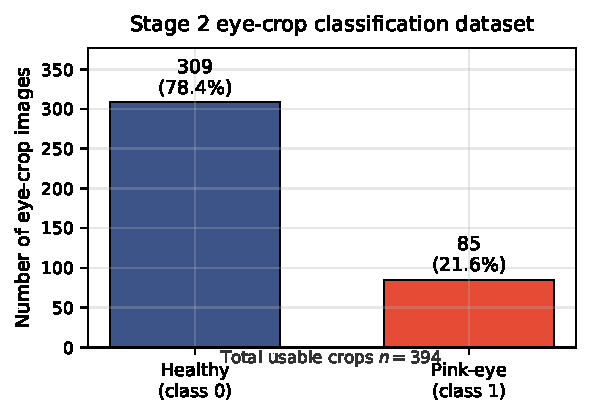
\includegraphics[width=0.82\linewidth]{figures/dataset_distribution.pdf}
  \caption{Class distribution of usable Stage~2 eye crops ($n{=}394$):
    309 healthy (78.4\,\%) and 85 pinkeye (21.6\,\%), matching folder labels
    after YOLO cropping.}
  \label{fig:dataset_dist}
\end{figure}

\subsection{Main Classification Benchmark}
\label{subsec:main_benchmark}

Table~\ref{tab:benchmark} lists 5-fold mean$\,\pm\,$std performance under
the full augmentation configuration (policy~(i)). Figure~\ref{fig:f1bar}
visualises mean F1$_{\mathrm{PE}}$ with error bars using the same
fold-wise summaries as Table~\ref{tab:benchmark}.

\begin{table*}[t]
  \caption{Stage~2 classification under full augmentation (5-fold
    mean$\,\pm\,$std). Best per column in bold.}
  \label{tab:benchmark}
  \centering
  \setlength{\tabcolsep}{5pt}
  \begin{tabular}{lcccccc}
    \toprule
    \textbf{Model}
      & \textbf{Accuracy}
      & \textbf{Bal.\ Acc.}
      & \textbf{Precision\textsubscript{PE}}
      & \textbf{Recall\textsubscript{PE}}
      & \textbf{F1\textsubscript{PE}}
      & \textbf{ROC-AUC} \\
    \midrule
    ResNet18
      & $0.9569 \pm 0.0144$
      & $0.9342 \pm 0.0289$
      & $0.9094 \pm 0.0619$
      & $0.8941 \pm 0.0644$
      & $0.8992 \pm 0.0342$
      & $\mathbf{0.9867 \pm 0.0117}$ \\
    EfficientNet-B0
      & $0.9568 \pm 0.0114$
      & $\mathbf{0.9383 \pm 0.0297}$
      & $0.8980 \pm 0.0393$
      & $\mathbf{0.9059 \pm 0.0671}$
      & $0.9000 \pm 0.0279$
      & $0.9829 \pm 0.0122$ \\
    CNN+Transformer
      & $0.9239 \pm 0.0235$
      & $0.9132 \pm 0.0215$
      & $0.7934 \pm 0.0928$
      & $0.8941 \pm 0.0492$
      & $0.8369 \pm 0.0429$
      & $0.9681 \pm 0.0327$ \\
    \textbf{Strong CNN+Transformer}
      & $\mathbf{0.9594 \pm 0.0106}$
      & $0.9358 \pm 0.0229$
      & $\mathbf{0.9251 \pm 0.0795}$
      & $0.8941 \pm 0.0644$
      & $\mathbf{0.9051 \pm 0.0214}$
      & $0.9850 \pm 0.0024$ \\
    \bottomrule
  \end{tabular}
  \\[2pt]
  \small PE $=$ pinkeye (minority class). Metrics aggregated from five-fold
    validation.
\end{table*}

\begin{figure}[t]
  \centering
  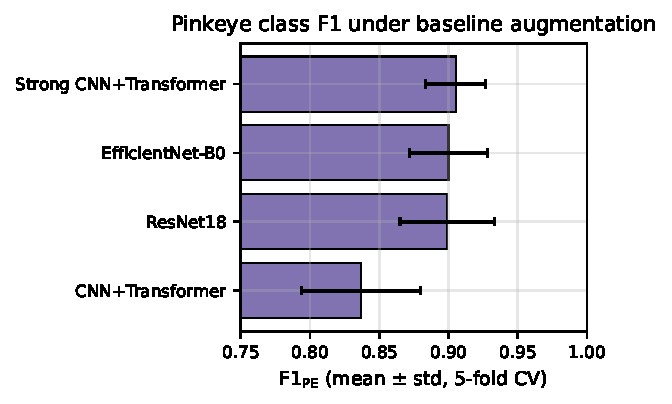
\includegraphics[width=\linewidth]{figures/benchmark_f1_pinkeye.pdf}
  \caption{Mean$\,\pm\,$std F1$_{\mathrm{PE}}$ under full augmentation,
    replotted from the same statistics as Table~\ref{tab:benchmark}.}
  \label{fig:f1bar}
\end{figure}

\subsection{Fold-Level Behaviour and Confusion Matrix}
Table~\ref{tab:per_fold} gives per-fold accuracy and F1$_{\mathrm{PE}}$
for ResNet18 and Strong CNN+Transformer. Table~\ref{tab:confusion}
aggregates confusion counts across folds for Strong CNN+Transformer.

\begin{table}[h]
  \caption{Per-fold accuracy and F1$_{\mathrm{PE}}$ (full augmentation).}
  \label{tab:per_fold}
  \centering
  \begin{tabular}{ccccc}
    \toprule
    \multirow{2}{*}{\textbf{Fold}}
      & \multicolumn{2}{c}{\textbf{ResNet18}}
      & \multicolumn{2}{c}{\textbf{Strong CNN+T}} \\
    \cmidrule(lr){2-3}\cmidrule(lr){4-5}
      & Acc. & F1\textsubscript{PE}
      & Acc. & F1\textsubscript{PE} \\
    \midrule
    1 & 0.9494 & 0.8889 & 0.9494 & 0.8889 \\
    2 & 0.9620 & 0.9143 & 0.9747 & 0.9412 \\
    3 & 0.9747 & 0.9412 & 0.9494 & 0.8889 \\
    4 & 0.9367 & 0.8485 & 0.9620 & 0.9032 \\
    5 & 0.9615 & 0.9032 & 0.9615 & 0.9032 \\
    \midrule
    Mean & 0.9569 & 0.8992 & 0.9594 & 0.9051 \\
    Std  & 0.0144 & 0.0342 & 0.0106 & 0.0214 \\
    \bottomrule
  \end{tabular}
\end{table}

\begin{table}[h]
  \caption{Aggregated confusion matrix for Strong CNN+Transformer (sum over
    validation folds; total samples $=394$).}
  \label{tab:confusion}
  \centering
  \begin{tabular}{ccc}
    \toprule
    \multirow{2}{*}{\textbf{True $\backslash$ Pred}}
      & \textbf{Healthy}
      & \textbf{Pink-eye} \\
    \midrule
    \textbf{Healthy}  & 302 & \phantom{0}7 \\
    \textbf{Pink-eye} & \phantom{0}9 & 76 \\
    \bottomrule
  \end{tabular}
\end{table}

Fold-level confusion matrices, ROC curves, and learning curves were saved
with the original GPU experiments but are omitted here for brevity.

\subsection{Augmentation Comparisons}

\subsubsection{Removing Colour Augmentation}
Table~\ref{tab:no_color_delta} contrasts policy~(i) (full augmentation)
with policy~(ii) (no colour) using five-fold mean F1$_{\mathrm{PE}}$ and
accuracy.

\begin{table}[t]
  \caption{Effect of removing colour-related augmentation: mean
    F1$_{\mathrm{PE}}$ and accuracy (5-fold mean).}
  \label{tab:no_color_delta}
  \centering
  \begin{tabular}{lcccc}
    \toprule
    \textbf{Model}
      & \textbf{F1\textsubscript{PE} (full)}
      & \textbf{F1\textsubscript{PE} (no-col)}
      & \textbf{$\Delta$F1}
      & \textbf{$\Delta$Acc} \\
    \midrule
    ResNet18
      & 0.8992 & \textbf{0.9190} & \textbf{+0.0198} & +0.0076 \\
    EfficientNet-B0
      & \textbf{0.9000} & 0.8721 & $-$0.0279 & $-$0.0152 \\
    CNN+Transformer
      & 0.8369 & 0.8272 & $-$0.0097 & $-$0.0001 \\
    Strong CNN+T
      & \textbf{0.9051} & 0.8672 & $-$0.0379 & $-$0.0153 \\
    \bottomrule
  \end{tabular}
\end{table}

Removing colour augmentation improved ResNet18 but reduced F1$_{\mathrm{PE}}$
for EfficientNet-B0 and both hybrid models, indicating an interaction
between architecture and augmentation strength.

\subsubsection{Gaussian Noise Ablation}
Table~\ref{tab:ablation_noise} compares no-colour training with and without
Gaussian noise by juxtaposing policy~(ii) and policy~(iii) means under the
same protocol.

\begin{table}[h]
  \caption{Gaussian noise ablation: mean F1$_{\mathrm{PE}}$.
    $\Delta$ is flip+rotation (no noise) minus no-colour+noise.}
  \label{tab:ablation_noise}
  \centering
  \begin{tabular}{lccc}
    \toprule
    \textbf{Model}
      & \textbf{No-col+noise}
      & \textbf{Flip+rot}
      & \textbf{$\Delta$F1\textsubscript{PE}} \\
    \midrule
    ResNet18          & 0.9190 & 0.8979 & $-$0.0210 \\
    EfficientNet-B0   & 0.8721 & 0.8518 & $-$0.0202 \\
    Strong CNN+T      & 0.8672 & \textbf{0.8788} & \textbf{+0.0117} \\
    \bottomrule
  \end{tabular}
\end{table}

\subsubsection{Minority-Only Augmentation}
Table~\ref{tab:ablation_minority} summarises mean F1$_{\mathrm{PE}}$ under
no-colour+noise, all-class flip+rotation, and minority-only
flip+rotation under the same protocol.

\begin{table}[h]
  \caption{Minority-only versus all-class geometric augmentation
    (mean F1$_{\mathrm{PE}}$).}
  \label{tab:ablation_minority}
  \centering
  \setlength{\tabcolsep}{4pt}
  \begin{tabular}{lcccc}
    \toprule
    \textbf{Model}
      & \textbf{No-col+noise}
      & \textbf{Flip+rot (all)}
      & \textbf{Flip+rot (min.)}
      & \textbf{Best setting} \\
    \midrule
    ResNet18
      & \textbf{0.9190} & 0.8979 & 0.9060 & no-col+noise \\
    EfficientNet-B0
      & \textbf{0.8721} & 0.8518 & 0.8624 & no-col+noise \\
    Strong CNN+T
      & 0.8672 & \textbf{0.8788} & 0.8582 & flip+rot (all) \\
    \bottomrule
  \end{tabular}
\end{table}

\subsubsection{Best Model per Configuration}
Table~\ref{tab:full_comparison} condenses the best mean accuracy and
F1$_{\mathrm{PE}}$ per augmentation regime.

\begin{table*}[t]
  \caption{Best mean accuracy / F1$_{\mathrm{PE}}$ by augmentation
    regime (5-fold means).}
  \label{tab:full_comparison}
  \centering
  \begin{tabular}{llcc}
    \toprule
    \textbf{Configuration}
      & \textbf{Best model}
      & \textbf{Accuracy}
      & \textbf{F1\textsubscript{PE}} \\
    \midrule
    Full augmentation (colour + affine)
      & Strong CNN+Transformer
      & $0.9594 \pm 0.0106$
      & $0.9051 \pm 0.0214$ \\
    No colour (+ Gaussian noise)
      & ResNet18
      & $0.9645 \pm 0.0165$
      & $0.9190 \pm 0.0374$ \\
    Geometric only (flip + rotation)
      & ResNet18
      & $0.9543 \pm 0.0147$
      & $0.8979 \pm 0.0312$ \\
    Minority-only augmentation
      & ResNet18
      & $0.9594 \pm 0.0105$
      & $0.9060 \pm 0.0282$ \\
    \bottomrule
  \end{tabular}
\end{table*}

Under the primary full-augmentation benchmark, Strong CNN+Transformer
delivers the highest mean accuracy and F1$_{\mathrm{PE}}$. Under the
no-colour policy, ResNet18 achieves a higher mean F1$_{\mathrm{PE}}$
(0.9190) but with larger fold-wise dispersion ($\pm 0.0374$ vs.\
$\pm 0.0214$ for Strong CNN+Transformer under full augmentation).

\subsection{DDPM-Based Synthetic Augmentation (Pilot)}
\label{subsec:ddpm_pilot}

To probe generative remedies for class imbalance, we trained a
class-conditional denoising diffusion probabilistic model (DDPM)
\cite{ho2020ddpm} to synthesise eye crops labelled \emph{healthy} or
\emph{pinkeye}, matching the Stage~2 taxonomy. The diffusion training
configuration used batch size~16, $T{=}10{,}000$ noise steps, and
2048~epochs. Figure~\ref{fig:ddpm_qualitative} shows representative
real crops from the classification pool next to synthetic draws from the
trained generators for each class.

The intended workflow is to screen synthetic samples for anatomical and
pathology plausibility, then add accepted images to training folds in a
controlled mix with real data, re-run the stratified 5-fold Stage~2
benchmarks, and compare minority-class recall and F1$_{\mathrm{PE}}$
against real-only training. Those mixed training runs are preparatory:
all tables above report models trained only on real eye crops.

\begin{figure*}[t]
  \centering
  \begin{minipage}[t]{0.48\textwidth}
    \centering
    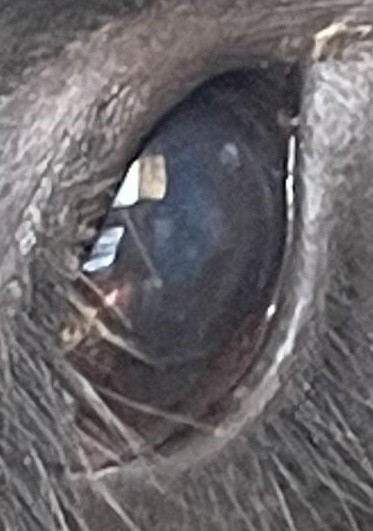
\includegraphics[width=\linewidth]{figures/ddpm_healthy_original.jpg}\\[2pt]
    \footnotesize (a)~Healthy crop (real)
  \end{minipage}\hfill
  \begin{minipage}[t]{0.48\textwidth}
    \centering
    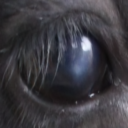
\includegraphics[width=\linewidth]{figures/ddpm_healthy_synthetic.png}\\[2pt]
    \footnotesize (b)~Healthy (DDPM synthetic)
  \end{minipage}\\[10pt]
  \begin{minipage}[t]{0.48\textwidth}
    \centering
    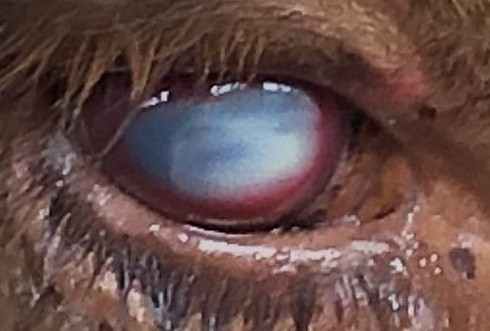
\includegraphics[width=\linewidth]{figures/ddpm_pinkeye_original.jpg}\\[2pt]
    \footnotesize (c)~Pinkeye crop (real)
  \end{minipage}\hfill
  \begin{minipage}[t]{0.48\textwidth}
    \centering
    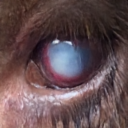
\includegraphics[width=\linewidth]{figures/ddpm_pinkeye_synthetic.png}\\[2pt]
    \footnotesize (d)~Pinkeye (DDPM synthetic)
  \end{minipage}
  \caption{Qualitative comparison of real Stage~2 crops and class-conditional
    DDPM samples (pilot augmentation study). Training used batch size~16,
    $T{=}10{,}000$, and 2048~epochs.}
  \label{fig:ddpm_qualitative}
\end{figure*}

\section{Discussion}
\label{sec:discussion}

\subsection{Architecture Rankings and Augmentation Interactions}
Strong CNN+Transformer leads on mean accuracy and F1$_{\mathrm{PE}}$ when
the richer augmentation policy is used, while ResNet18 achieves the
best mean ROC-AUC in Table~\ref{tab:benchmark} and the best mean
F1$_{\mathrm{PE}}$ under the no-colour regime (Table~\ref{tab:full_comparison}).
The ablations indicate that colour and affine regularisation in policy~(i)
particularly benefit the deeper CNN and hybrid models, whereas the
shallow ResNet benefits when colour perturbations are omitted.

\subsection{Qualitative Attribution}
Gradient-based Grad-CAM visualisations \cite{selvaraju2017gradcam} were
computed for the CNN baselines during training. Illustrative overlays are
not reproduced in this manuscript; qualitatively, saliency tended to align
with conjunctival and peripheral corneal regions on pinkeye crops, consistent
with clinical presentation.

\subsection{Limitations and Future Work}
The dataset size (85 pinkeye crops) limits generalisation claims. A
class-conditional DDPM for synthetic augmentation was trained
\cite{ho2020ddpm}; Figure~\ref{fig:ddpm_qualitative} illustrates sample
quality relative to real crops. Systematic Stage~2 fine-tuning with
curated synthetic augmentation and reporting against the benchmark protocol
remains future work. Broader directions include larger multi-site
collections, severity grading, and external validation.

\section*{Acknowledgements}
The authors acknowledge computing resources provided by [HPC Centre].
Step~1 and Step~2 GPU jobs used the institution's SLURM-managed cluster with
CUDA modules provisioned by the computing centre.

\bibliographystyle{IEEEtran}
\begin{thebibliography}{10}

\bibitem{roboflow_eye}
I.\ Khazrak,
``Eye Detection Dataset (v3),''
Roboflow Universe, 2026.
[Online]. Available: \url{https://universe.roboflow.com/imans-workspace-rsc4n/eye-detection-fayd6}

\bibitem{advisor_summary}
Internal technical memorandum, Cattle Pinkeye Detection project,
Mar.\ 2026 (dataset inventory and crop statistics).

\bibitem{he2016resnet}
K.\ He, X.\ Zhang, S.\ Ren, and J.\ Sun,
``Deep Residual Learning for Image Recognition,''
in \emph{Proc.\ IEEE/CVF CVPR}, 2016, pp.\ 770--778.

\bibitem{tan2019efficientnet}
M.\ Tan and Q.\ V.\ Le,
``EfficientNet: Rethinking Model Scaling for Convolutional Neural Networks,''
in \emph{Proc.\ ICML}, 2019, pp.\ 6105--6114.

\bibitem{loshchilov2018adamw}
I.\ Loshchilov and F.\ Hutter,
``Decoupled Weight Decay Regularization,''
in \emph{Proc.\ ICLR}, 2019.

\bibitem{rw2019timm}
R.\ Wightman,
``PyTorch Image Models,''
GitHub, 2019.
[Online]. Available: \url{https://github.com/rwightman/pytorch-image-models}

\bibitem{selvaraju2017gradcam}
R.\ R.\ Selvaraju, M.\ Cogswell, A.\ Das, R.\ Vedantam, D.\ Parikh,
and D.\ Batra,
``Grad-CAM: Visual Explanations from Deep Networks via
Gradient-Based Localization,''
in \emph{Proc.\ IEEE ICCV}, 2017, pp.\ 618--626.

\bibitem{ultralytics2023yolov8}
G.\ Jocher, A.\ Chaurasia, and J.\ Qiu,
``Ultralytics YOLOv8,''
GitHub, 2023.
[Online]. Available: \url{https://github.com/ultralytics/ultralytics}

\bibitem{ho2020ddpm}
J.\ Ho, A.\ Jain, and P.\ Abbeel,
``Denoising Diffusion Probabilistic Models,''
in \emph{Advances in Neural Information Processing Systems (NeurIPS)},
vol.\ 33, 2020, pp.\ 6840--6851.

\end{thebibliography}

\end{document}
